\subsection{Composite}
\subsubsection{Định nghĩa}
Composite là một mẫu thiết kế thuộc nhóm cấu trúc (structural design pattern) trong lập trình hướng đối tượng. Mẫu thiết kế này cho phép bạn tạo ra cấu trúc cây đặc biệt, gồm các đối tượng con và đối tượng tổng hợp chung một giao diện chung. Composite cho phép các đối tượng con và đối tượng tổng hợp được xử lý một cách đồng nhất, không phân biệt.
\subsubsection{Cách sử dụng}
Hãy sử dụng khi:
\begin{itemize}
    \item Khi bạn muốn thực hiện các hoạt động chung cho tất cả các đối tượng trong cây mà không cần kiểm tra kiểu của chúng.
    \item Khi bạn muốn tạo ra các đối tượng trong các cấu trúc cây để biểu diễn hệ thống phân lớp.
\end{itemize}
\subsubsection{Cấu trúc}
\begin{center}
    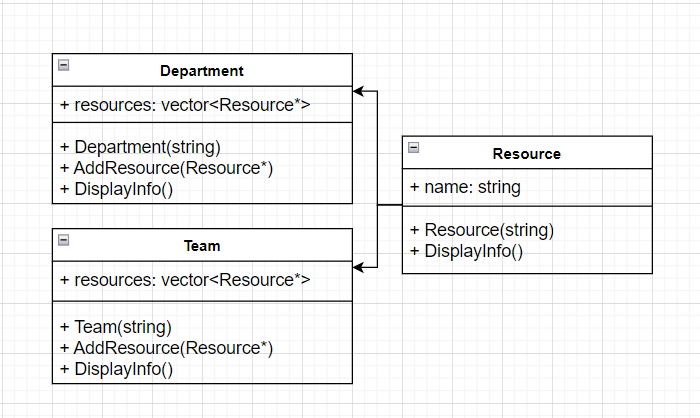
\includegraphics[scale=0.7]{image/structural/composite.png}
\end{center}
Các thành phần chính bao gồm:
\begin{itemize}
    \item Component: là một interface hoặc abstract class định nghĩa chung cho các thành phần con tham gia trong cây.
    \item Leaf: là các lớp thực hiện các phương thức của component, không có subclass.
    \item Composite: lưu trữ các Leaf và các phương thức của Component đồng thời ủy nhiệm nhiệm vụ thực hiện cho các Leaf.
\end{itemize}
\subsubsection{Ưu điểm và Nhược điểm}
Ta có các ưu và nhược điểm dễ thấy sau:\\\\
Ưu điểm:
\begin{itemize}
    \item Composite cho phép bạn xử lý các đối tượng con và đối tượng tổng hợp theo cách thống nhất, mà không phải phân biệt giữa chúng.
    \item Bạn có thể dễ dàng thêm mới các đối tượng con vào cây mà không ảnh hưởng đến cấu trúc tổng thể của cây.
\end{itemize}
Nhược điểm:
\begin{itemize}
    \item Có thể gây ra hiệu năng giảm đối với các cây rất lớn do việc duyệt qua toàn bộ cấu trúc.
\end{itemize}
\subsubsection{Code Example}
\begin{itemize}
    \item Một công ty có các rất nhiều bộ phận liên kết với nhau tạo thành một cây hoàn chỉnh.
\end{itemize}
\begin{lstlisting}
#include <iostream>
#include <string>
#include <vector>

namespace Company {
    class Resource {
    protected:
        std::string name;

    public:
        Resource(const std::string& name) : name(name) {}

        virtual void DisplayInfo() const = 0;
    };

    class Department : public Resource {
    private:
        std::vector<Resource*> resources;

    public:
        Department(const std::string& name) : Resource(name) {}

        void AddResource(Resource* resource) {
            resources.push_back(resource);
        }

        void DisplayInfo() const override {
            std::cout << "Department: " << name << std::endl;
            for (const auto& resource : resources) {
                resource->DisplayInfo();
            }
        }
    };

    class Team : public Resource {
    private:
        std::vector<Resource*> resources;

    public:
        Team(const std::string& name) : Resource(name) {}

        void AddResource(Resource* resource) {
            resources.push_back(resource);
        }

        void DisplayInfo() const override {
            std::cout << "Team: " << name << std::endl;
            for (const auto& resource : resources) {
                resource->DisplayInfo();
            }
        }
    };

    class Employee : public Resource {
    private:
        std::string position;

    public:
        Employee(const std::string& name, const std::string& position) : Resource(name), position(position) {}

        void DisplayInfo() const override {
            std::cout << "Employee: " << name << " (Position: " << position << ")" << std::endl;
        }
    };

    class Project : public Resource {
    private:
        std::string status;

    public:
        Project(const std::string& name, const std::string& status) : Resource(name), status(status) {}

        void DisplayInfo() const override {
            std::cout << "Project: " << name << " (Status: " << status << ")" << std::endl;
        }
    };
}

int main() {
    using namespace Company;

    Department* developmentDepartment = new Department("Development Department");

    Team* team1 = new Team("Team 1");
    Employee* employee1 = new Employee("John Doe", "Software Engineer");
    Employee* employee2 = new Employee("Jane Smith", "UI/UX Designer");
    team1->AddResource(employee1);
    team1->AddResource(employee2);

    Team* team2 = new Team("Team 2");
    Employee* employee3 = new Employee("Mike Johnson", "Backend Developer");
    Employee* employee4 = new Employee("Emily Davis", "Frontend Developer");
    team2->AddResource(employee3);
    team2->AddResource(employee4);

    developmentDepartment->AddResource(team1);
    developmentDepartment->AddResource(team2);

    Project* project1 = new Project("Project A", "In Progress");
    Project* project2 = new Project("Project B", "Completed");

    developmentDepartment->AddResource(project1);
    developmentDepartment->AddResource(project2);

    developmentDepartment->DisplayInfo();

    delete developmentDepartment;
    delete team1;
    delete team2;
    delete employee1;
    delete employee2;
    delete employee3;
    delete employee4;
    delete project1;
    delete project2;

    return 0;
}

\end{lstlisting}
Ở hàm main, ta tạo team1 và thêm 2 nhân viên vào đó. Ta tạo team 2 và thêm 2 nhân viên vào đó. Bộ phận phát triển thêm 2 team này vào nó. Bộ phận phát triển cũng thêm vào 2 dư án vừa được tạo. Sau cùng hiển thị ra toàn bộ.\\
\newline
\textbf{Kết quả:}
\begin{lstlisting}
Department: Development Department
Team: Team 1
Employee: John Doe (Position: Software Engineer)
Employee: Jane Smith (Position: UI/UX Designer)
Team: Team 2
Employee: Mike Johnson (Position: Backend Developer)
Employee: Emily Davis (Position: Frontend Developer)
Project: Project A (Status: In Progress)
Project: Project B (Status: Completed)

\end{lstlisting}
\subsubsection{Các Pattern liên quan}
\begin{itemize}
    \item Builder: kết hợp với builder để tạo ra cây phức tạp nhiều tầng.
    \item Chain of Responsibility: thường phối hợp chung với Composite có thể dễ dàng thấy vì tính tương đồng ở cấu trúc.
    \item Dùng Iterator để duyệt con.
    \item Dùng Visitor để thực hiện hành động đặc biệt trên toàn bộ cây.
    \item Flyweight: tiết kiệm dung lượng ram do việc tạo ra cây khá tốn bộ nhớ.
    \item Dùng Decorator để trang trí các thành phần con nếu cần.
    \item Dùng Prototype để clone() con hoặc clone() cả cây.
\end{itemize}